\documentclass{article}
\usepackage[utf8]{inputenc}
\usepackage[papersize={8.5in,11in},margin=0.8in]{geometry}
\usepackage{xcolor}
\usepackage{color, colortbl}
\usepackage{graphicx}
\usepackage{tikz}
\usepackage{amssymb}
\usepackage{amsmath}
\usetikzlibrary{positioning}
\usetikzlibrary{graphs,graphs.standard}


\title{CS520 Written HW 3}
\author{John Caruthers}
\date\today

\begin{document}
\maketitle

\begin{itemize}
    \item[1.] Draw the shortest path tree (SPT) on the following weight directed graph, starting from \textbf{node A}.
        \begin{center}
            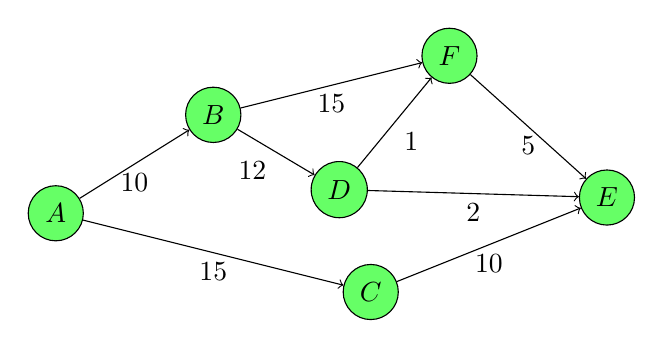
\begin{tikzpicture}
                [dot/.style = {minimum size = 0.7cm, draw, fill=green!60, circle}]
    
                \node[dot] (f) at (1,0) {$F$};
                \node[dot] (a) at (-4,-2) {$A$};
                \node[dot] (c) at (0,-3) {$C$};
                \node[dot] (b) at (-2,-0.75) {$B$};
                \node[dot] (d) at (-0.4,-1.7) {$D$};
                \node[dot] (e) at (3, -1.8) {$E$};
    
                \draw[->] (a) to node[below] {10} (b);
                \draw[->] (a) to node[below] {15} (c);
                \draw[->] (b) to node[below left] {12} (d);
                \draw[->] (c) to node[below] {10} (e);
                \draw[->] (b) to node[below] {15} (f);
                \draw[->] (d) to node[below] {2} (e);
                \draw[->] (d) to node[below right] {1} (f);
                \draw[->] (f) to node[below] {5} (e);
                % \draw[->,line width=3pt, color=purple] (c) to node[below] {3} (d);                
            \end{tikzpicture}
        \end{center}

        Resulting shortest path tree table
        
        \begin{centering}
            \begin{tabular}{|c|c|c|}
                \hline
                \emph{v} & edge to & dist to\\
                \hline
                A & - & 0\\
                \hline
                B & A & 10\\
                \hline
                C & A & 15\\
                \hline
                D & B & 22\\
                \hline
                E & D & 23\\
                \hline
                F & D & 24\\
                \hline
            \end{tabular}
        \end{centering}

        Resulting shortest path tree graph

        \begin{center}
            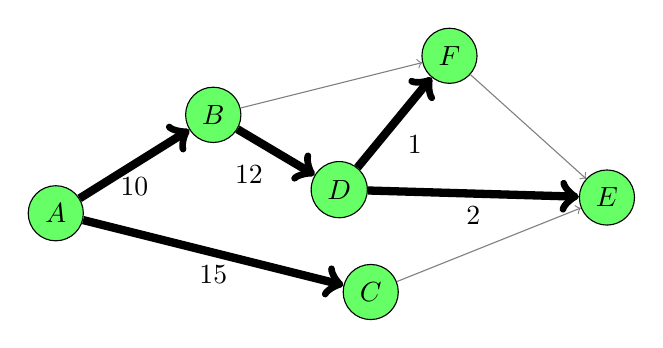
\begin{tikzpicture}
                [dot/.style = {minimum size = 0.7cm, draw, fill=green!60, circle}]
    
                \node[dot] (f) at (1,0) {$F$};
                \node[dot] (a) at (-4,-2) {$A$};
                \node[dot] (c) at (0,-3) {$C$};
                \node[dot] (b) at (-2,-0.75) {$B$};
                \node[dot] (d) at (-0.4,-1.7) {$D$};
                \node[dot] (e) at (3, -1.8) {$E$};
    
                \draw[->,line width=3pt] (a) to node[below] {10} (b);
                \draw[->,line width=3pt] (a) to node[below] {15} (c);
                \draw[->,line width=3pt] (b) to node[below left] {12} (d);
                \draw[->,color=gray] (c) to node[below] {} (e);
                \draw[->,color=gray] (b) to node[below] {} (f);
                \draw[->,line width=3pt] (d) to node[below] {2} (e);
                \draw[->,line width=3pt] (d) to node[below right] {1} (f);
                \draw[->,color=gray] (f) to node[below] {} (e);
                % \draw[->,line width=3pt, color=purple] (c) to node[below] {3} (d);                
            \end{tikzpicture}
        \end{center}
        
\end{itemize}

\end{document}
